\documentclass[times, utf8, diplomski]{fer}
\usepackage{booktabs}
\usepackage[final]{pdfpages}

\begin{document}

% TODO: Navedite broj rada.
\thesisnumber{2345}

\title{Proceduralno generiranje trave i niskog raslinja}
\author{Mihael Međan}

\maketitle

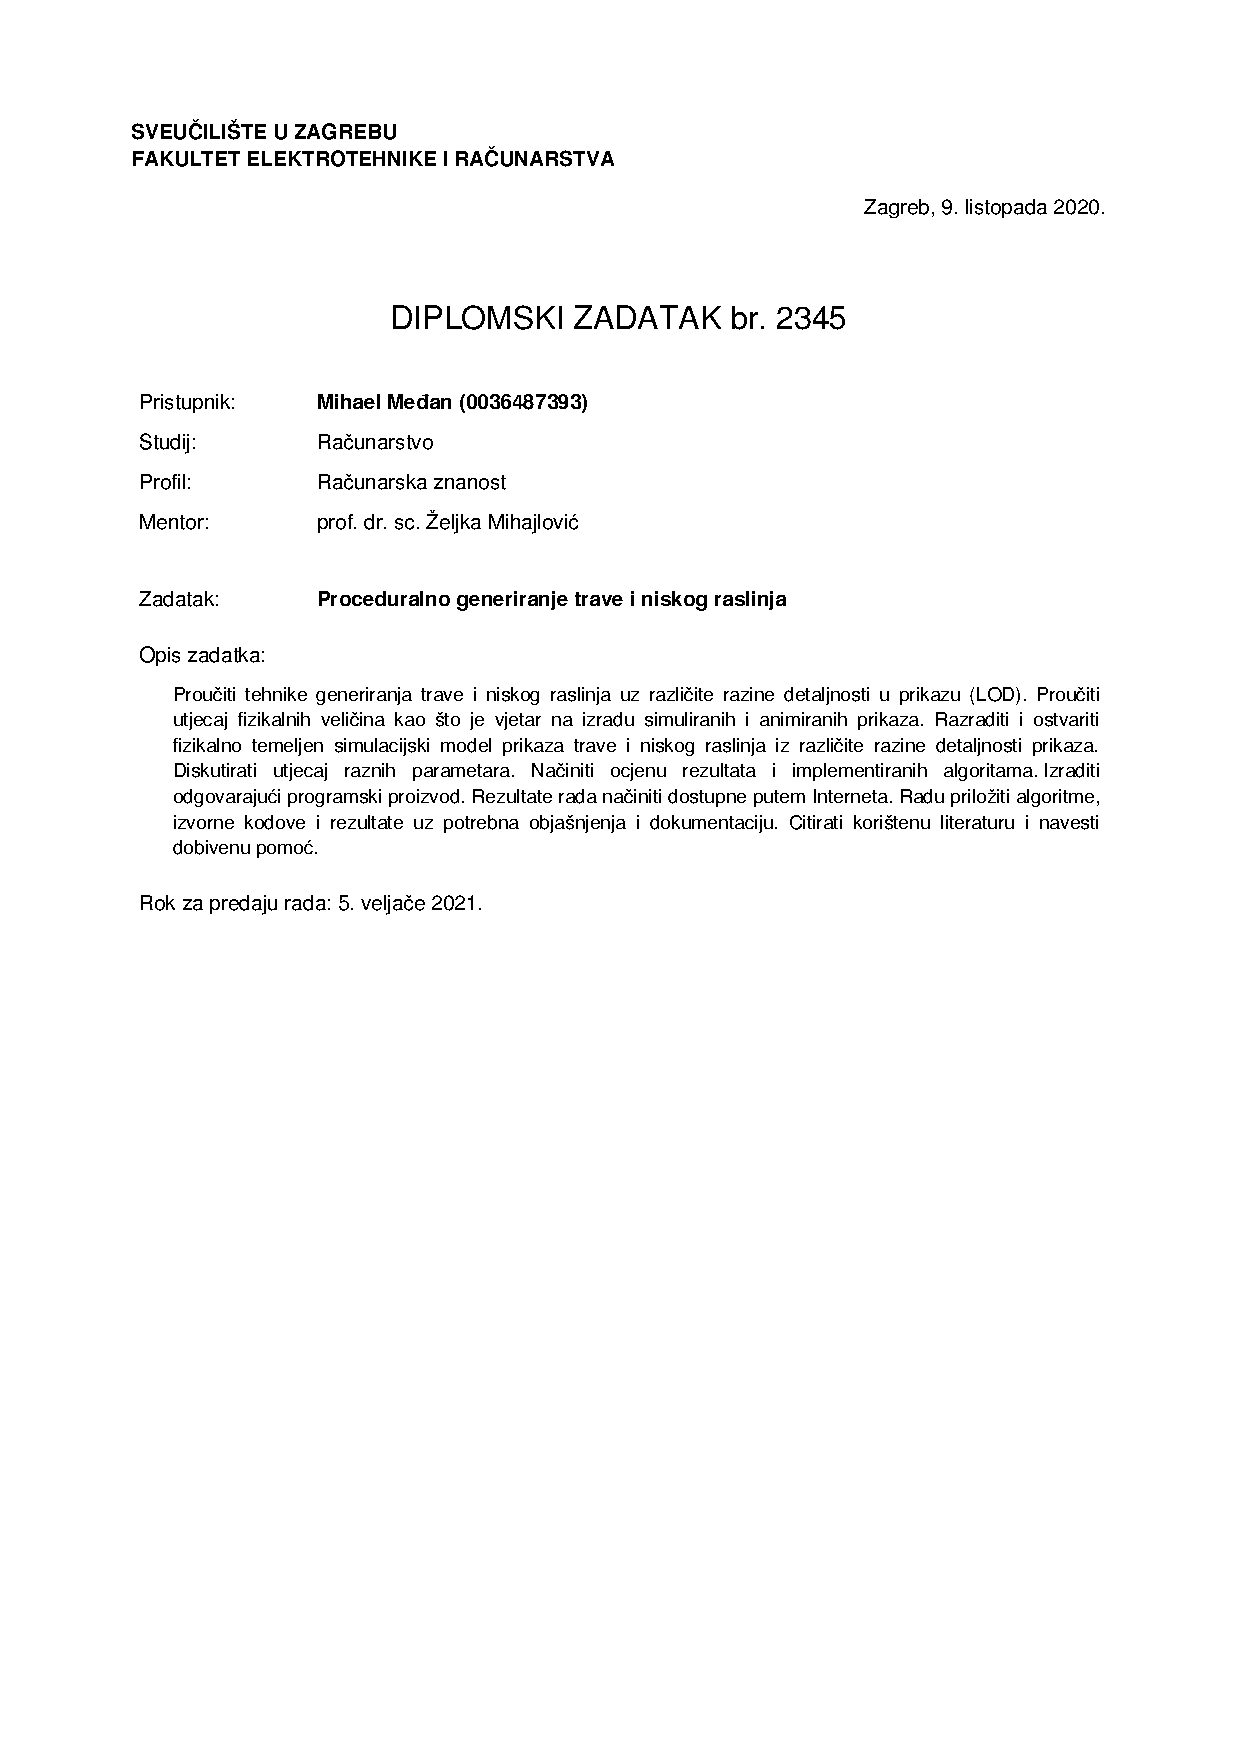
\includepdf[pages=-,offset=0 -75]{hr_0036487393_56.pdf}

\zahvala{}

\tableofcontents

\chapter{Uvod}
Uvod rada. Nakon uvoda dolaze poglavlja u kojima se obrađuje tema.

\chapter{Generiranje modela trave i niskog raslinja}
\section{Osnovni pristup generiranju modela}


\section{Generiranje točaka i poligona modela biljaka}
Tocke i poligoni

\subsection{Generiranje modela uz različitu razinu detalja}
LOD

\section{Povezivanje generiranih podataka i njihov prikaz}
Povezivanje i prikaz

\section{Programska implementacija generiranja i prikaza}
Tehnicka implementacija

\section{Primjer korištenja razvijenog programa za generiranje jednostavne proizvoljne biljke}
Primjer

\section{Dodavanje proizvoljnih atributa generiranim modelima}
Primjer

\section{Implementacija generiranja složenijih biljaka}
Wish do, would do, not :)

\chapter{Simulacijski model}
\section{Fizički model ponašanja biljke}
Kako bi se biljka kretala hehe

\section{Programski model fizičkog ponašanja}
Pojednostavljenje na jointove etc

\section{Programska implementacija fizičkog modela}
EZ

\section{Implementacije fizičkog ponašanja složenih biljaka}
drva buraz e

\chapter{Simulacija ponašanja generiranog modela}
\section{Povezivanje fizičkog modela sa generiranim prikazom modela}
skinning, buffers, bones

\section{Programska implementacija modela}
spajanje

\section{Utjecaj parametara na simulaciju}
wind, elasticity

\chapter{Ocjena rezultata}
\section{Realističnost prikaza}
\paragraph{}
Realističnost prikaza nije bila primarna zadaća ovog rada. Generirane biljke ne 
izgledaju osobito prirodno bez obzira na razinu detalja kojom su generirane.
\paragraph{}
Prvi razlog je primjena konstantnog sjenčanja poligona. U ovakvom načinu 
sjenčanja, normale za pojedine vrhove računamo kao normalu površine (poligona)
kojeg oni zatvaraju. Izračunata vrijednost normale se pripisuje svim vrhovima
poligona. Korištenjem konstantnog sjenčanja poligona postižemo jasno 
vidljivu granicu između pojedinih površina. Takav način prikaza, osim što je
vrlo brz u izvođenju, znatno je olakšao razvoj prezentiranog programskog 
rješenja jer daje programeru jasan uvid u poziciju pojedinih vrhova na ekranu
i njihovo ponašanje. 
\paragraph{}
Bez obzira na prednosti u razvoju koje ovakav pristup implicira, prikazani 
modeli izgledaju umjetno i izrazito su pravilni. Pravilnost modela je najveći
uzrok neprirodnog izgleda generiranih modela, jer na biljkama rijetko očekujemo
savršenu simetriju oko geometrijskih osi.
\paragraph{}
Drugi razlog je nedostatak detalja na generiranim modelima biljaka. Ovaj razlog 
dodatno naglašava pravilnost biljaka i smanjuje osjećaj realnosti prikaza.
Smanjenje broja detalja donijelo je iste prednosti kao i prethodni pristup - 
lakši razvoj i bolje performanse po cijenu realističnosti prikaza.
\paragraph{}
Treći razlog je izolacija prikaza. Biljke su prikazane kao centralni i jedini 
dio prikaza. Ovakav vakuum u prostoru dodatno naglašava oba prije spomenuta 
problema. Nedostatak simulacije atmosfere (prašina, distorzija zraka svjetlosti 
kao posljedica vlage u zraku itd.) uzrokuje dojam statičnosti biljaka bez
obzira na animirani prikaz ponašanja vjetra. Izostavak navedenih značajki, kao
i prethodna pojednostavljenja, olakšalo je razvoj programskog rješenja i 
oslobodilo vrijeme za ostvarenje kvalitetnije simulacije vjetra.

\subsection{Mogućnosti poboljšanja}
\paragraph{}
Problem sjenčanja može se riješiti primjenom nekog drugog načina sjenčanja 
modela. Naprimjer korištenje Gouraudovog sjenčanja. Korištenje ove metode 
sjenčanja eliminiralo bi vidljivost pojedinih vrhova na modelu i interpolacijom
između vrhova osiguralo gladak prijelaz između osjenčanih i ne osjenčanih 
dijelova modela. 
\paragraph{}
Biljke u stvarnosti rijetko imaju ikakve oštre bridove između svojih strana i 
zaglađivanje intenziteta osvjetljenja Gouraudovog sjenčanja između vrhova bi 
rezultiralo uvjerljivijim prikazom kod modela generiranih u većoj razini 
detalja. Kod modela generiranih manjom razinom detalja, rubovi samog modela bi
ostali oštri iako je model zaglađen. Sraz između rubova i unutrašnjosti modela
može uzrokovati smanjenje realističnosti prikaza.
\paragraph{}
Dodavanje malih varijacija kod generiranja modela poboljšalo bi realističnost 
prikaza. Mali istupi točaka od centra simetrije dali bi biljkama prirodniji
izgled uvođenjem nesavršenosti i raznovrsnosti biljaka. Osim dodavanja istupa
u poziciji točaka u modelu, istupi se mogu dodati i na boje pojedinih površina,
gdje bi neke površine bile više ili manje intenzivne boje od drugih. Dodavanje
boja u kombinaciji s Gouraudovim sjenčanjem dodatno bi pojačalo realističnost
prikaza.
\paragraph{}
Dodavanje varijacija je programski izrazito jednostavno za implementaciju ali
uzrokuje usporenje izvođenja, jer se svaki model zbog svoje unikatnosti mora
preslikati u memoriju grafičke kartice umjesto korištenja istog modela za sve 
biljke iste vrste. Kompromis se može postići na sredini - imati limitiran broj 
različitih modela iste vrste biljke koji se nasumično odabere za svaku biljku 
prilikom njenog kreiranja.
\paragraph{}
Dodavanje atmosferskih efekata na simulaciju bi uvelike pomoglo realističnosti
prikaza i dojmu živosti biljaka. Ovaj pristup riješavanju nerealističnosti 
prikaza je najkompleksniji od ponuđenih alternativa i zahtjeva razvoj nekolicine 
popratnih sustava, ali dao bi najveći doprinos realističnosti prikaza. Primjeri 
popratnih sustava koje je potrebno razviti uključuju: sustav ukrasnih čestica, 
sustav efekata nakon iscrtavanja (engl. \textit{post-processing effects}) i 
druge. 

\section{Realističnost fizičke simulacije}
\paragraph{}
Bez obzira na jednostavnost implementacije fizičke simulacije i snažne
pretpostavke uključene u nju, fizička simulacija daje zadovoljavajuće rezultate.
Ponašanje prati stvarno prirodno gibanje u tri dimenzije i ne potiče osjećaj 
umjetnosti ili ograničenosti prolaskom kroz prostor. Simulacija dobro modelira
utjecaj visine biljke na njezinu simulaciju na vjetru. 
\paragraph{}
Na udarima vjetra visoke biljke rade velike i snažne zamahe i polagano gube 
energiju za nastavak daljnjeg osciliranja. Niske biljke rade kraće zamahe ali 
većom frekvencijom.
\paragraph{}
Kod konstantnog puhanja, biljke osciliraju prema točki konvergencije sile 
puhanja, sile teže i sila otpora unutar stabljke. Visoke biljke očekivano imaju veću amplitudu i manju frekvenciju oko te točke od niskih biljaka.
\paragraph{}
Puhanje s naletima vjetra također daje realistične rezultate. Niske biljke u 
naletu vjetra se brzo poravnavaju prema točki konvergencije i osciliraju oko 
nje, a po prestanku puhanja osciliraju oko centra ravnoteže velikom 
frekvencijom. Visoke biljke imaju veću tromost i rade veće oscilacije oko točke
konvergencije vjetra i otpora biljke prilikom naleta vjetra. Kad vjetar 
prestane, naprave manje oscilacija oko centra ravnoteže prije nego vjetar 
ponovno počne.
\paragraph{}
Kad je simulacija vjetra realistična (takva da vjetar dolazi i prolazi u 
valovima - postepeno raste u snazi, i nakon toga postepeno opada u snazi) 
također imamo realističnu simulaciju. Visoke biljke održavaju smjer i neprestano 
osciliraju prema središtu između točaka centra ravnoteže otpora biljke, i 
konvergentne točke sile vjetra, ravnoteže i unutarnjeg otpora biljke. Niske 
biljke kod ovakvog vjetra djeluju kaotično i osciliraju velikom frekvencijom i 
amplitudom, sa središtem oscilacije koji vidno varira između konvergentne točke 
i centra ravnoteže biljke.

\subsection{Poboljšanje realističnosti simulacije}
better

\section{Ocjena brzine izvođenja}
\paragraph{}
Brzina izvođenja linearno opada s brojem simuliranih biljaka. Najveći utjecaj na 
brzinu izvođenja ima fizička simulacija. Generiranje biljaka se odvija na samom 
početku i nema nikakvog utjecaja na brzinu izvođenja nakon početnog perioda 
generiranja. Iscrtavanje je zbog jednostavnosti prikaza vrlo jeftino i usporava
izvođenje tek na velikom broju biljaka ili na vrlo visokoj razini detalja.

\subsection{Pristupi poboljšanju brzine izvođenja}
\paragraph{}
Fizička simulacija ima najveći utjecaj na brzinu izvođenja pa su prijedlozi za 
ubrzanje programskog rješenja fokusirani na taj dio.
\subsubsection{Paralelno izvođenje fizičke simulacije}
paralelism

\subsubsection{Smanjenje rezolucije simulacije i interpolacija rezultata}
nice

\subsubsection{Izračunavanje sličnosti modela i grupiranje izračuna}
bad

\chapter{Zaključak}
ma moze se sve buraz kad se oce

\bibliography{literatura}
\bibliographystyle{fer}

\begin{sazetak}
Sažetak na hrvatskom jeziku.

\kljucnerijeci{Ključne riječi, odvojene zarezima.}
\end{sazetak}

% TODO: Navedite naslov na engleskom jeziku.
\engtitle{Procedural generation of grass and low vegetation}
\begin{abstract}
Abstract.

\keywords{Keywords.}
\end{abstract}

\end{document}
